
\subsection{First Day TOPP Value Comparison} \label{ss:day1} %first day comparison

\begin{figure}
    \begin{center}
        \includegraphics[width=\textwidth]{img/first_day_values}
    \end{center}
    \caption{First day TOPP values obtained using (a) MCM v3.1, (b) CRI v2, \mbox{(c) MOZART-4}, (d) RADM2, (e) RACM, (f) RACM2, (g) CBM-IV and (h) CB05 mechanisms compared to the corresponding MCM v3.2 values.}
    \label{f:first_day}
\end{figure}

\begin{figure}
    \begin{center}
        \includegraphics[width=\textwidth]{img/Ox_tagged_budget_overlay_all_mechanisms}
    \end{center}
    \caption{\ce{O_x} production budgets allocated to individual VOCs using (a) MCM v3.2, \mbox{(b) MCM v3.1}, (c) CRI v2, (d) RADM2, (e) RACM, (f) RACM2, (g) MOZART-4, \mbox{(h) CBM-IV} and (i) CB05 mechanisms.}
    \label{f:Ox_tagged_budgets}
\end{figure}

The first day TOPP values calculated from each mechanism are compared to those calculated with the MCM v3.{2} in Figure \ref{f:first_day}. 
The reduced mechanisms generally match the MCM v3.2 first day TOPP values. 
However the TOPP values resulting from aromatic VOC degradation is lower in the reduced mechanisms.

Aromatic chemistry is difficult to represent in chemical mechanisms as many products, their yields and reactions are not known or are subject to uncertainties \citep{Vereecken:2012}. 
Thus, greater variation is expected between the aromatic VOC TOPP values.
The largest discrepancies are the zero TOPP values of toluene and xylene in RACM. 
This is unrealistic as aromatic VOCs contribute significantly to \ce{O_x} production \citep{Derwent:1998}. 
Section \ref{sss:RACM_aromatic} outlines the responsible chemistry.

The $2$-methylpropene first day TOPP values in RACM, RACM2, CBM-IV and CB05 indicate that its degradation is treated very differently to the MCM v3.2. 
The variation between RACM, RACM2 and MCM v3.2 arise from differences between the rate constants of $2$-methylpropene ozonolysis. 
These rate constants are derived from the IUPAC recommendations\citep{IUPAC_Site}, however RACM and RACM2 rate constants are an order of magnitude faster than the MCM v3.2.
This is the outcome of the rate constant being a weighted mean of all VOC ozonolysis rate constants represented as OLI in RACM and RACM2 \citep{Stockwell:1997, Goliff:2013}.
The resulting increased radical production leads to more \ce{O_x} production than in the MCM v3.2.

In CBM-IV, $2$-methylpropene is represented by the mechanism species ALD2 \citep{Hogo:1989}, which is a surrogate for aldehydes with more than one carbon atom. 
ALD2 reacts very quickly with OH forming \ce{CH3CO3}, leading to \ce{O_x} production. 
Furthermore, photolysis of ALD2 promotes radical and in turn \ce{O_x} production. 
This is not a degradation pathway for $2$-methylpropene in any other mechanism. 
The choice of $2$-methylpropene representation gives rise to more \ce{O_x} production than in the MCM v3.2.

$2$-methylpropene representation was updated in CB05 to \mbox{FORM + $3$ PAR}, where FORM represents formaldehyde and PAR the paraffin \ce{C-C} bond \citep{Yarwood:2005}. 
The initial oxidation reactions of formaldehyde are similar to ALD2 whilst PAR is a slow reacting species. 
This slows down the \ce{O_x} production resulting in lower \ce{O_x} production than in the MCM v3.2.

The first day TOPP values of many VOCs using CBM-IV and CB05 are lower than those of the MCM v3.2. 
This is related to lower \ce{O_x} production in CBM-IV and CB05, shown in Figure \ref{f:Ox_tagged_budgets}.
Lower \ce{O3} levels using CBM-IV and CB05 have also been noted in other modelling studies such as \citet{Luecken:2008, Emmerson:2009} and \citet{Saylor:2012}.
Analysis of the lower \ce{O_x} production is investigated in the following sections.

\subsection{TOPP Values Time Series} \label{ss:profiles} %TOPP time series of all species

\begin{figure}
    \begin{center}
        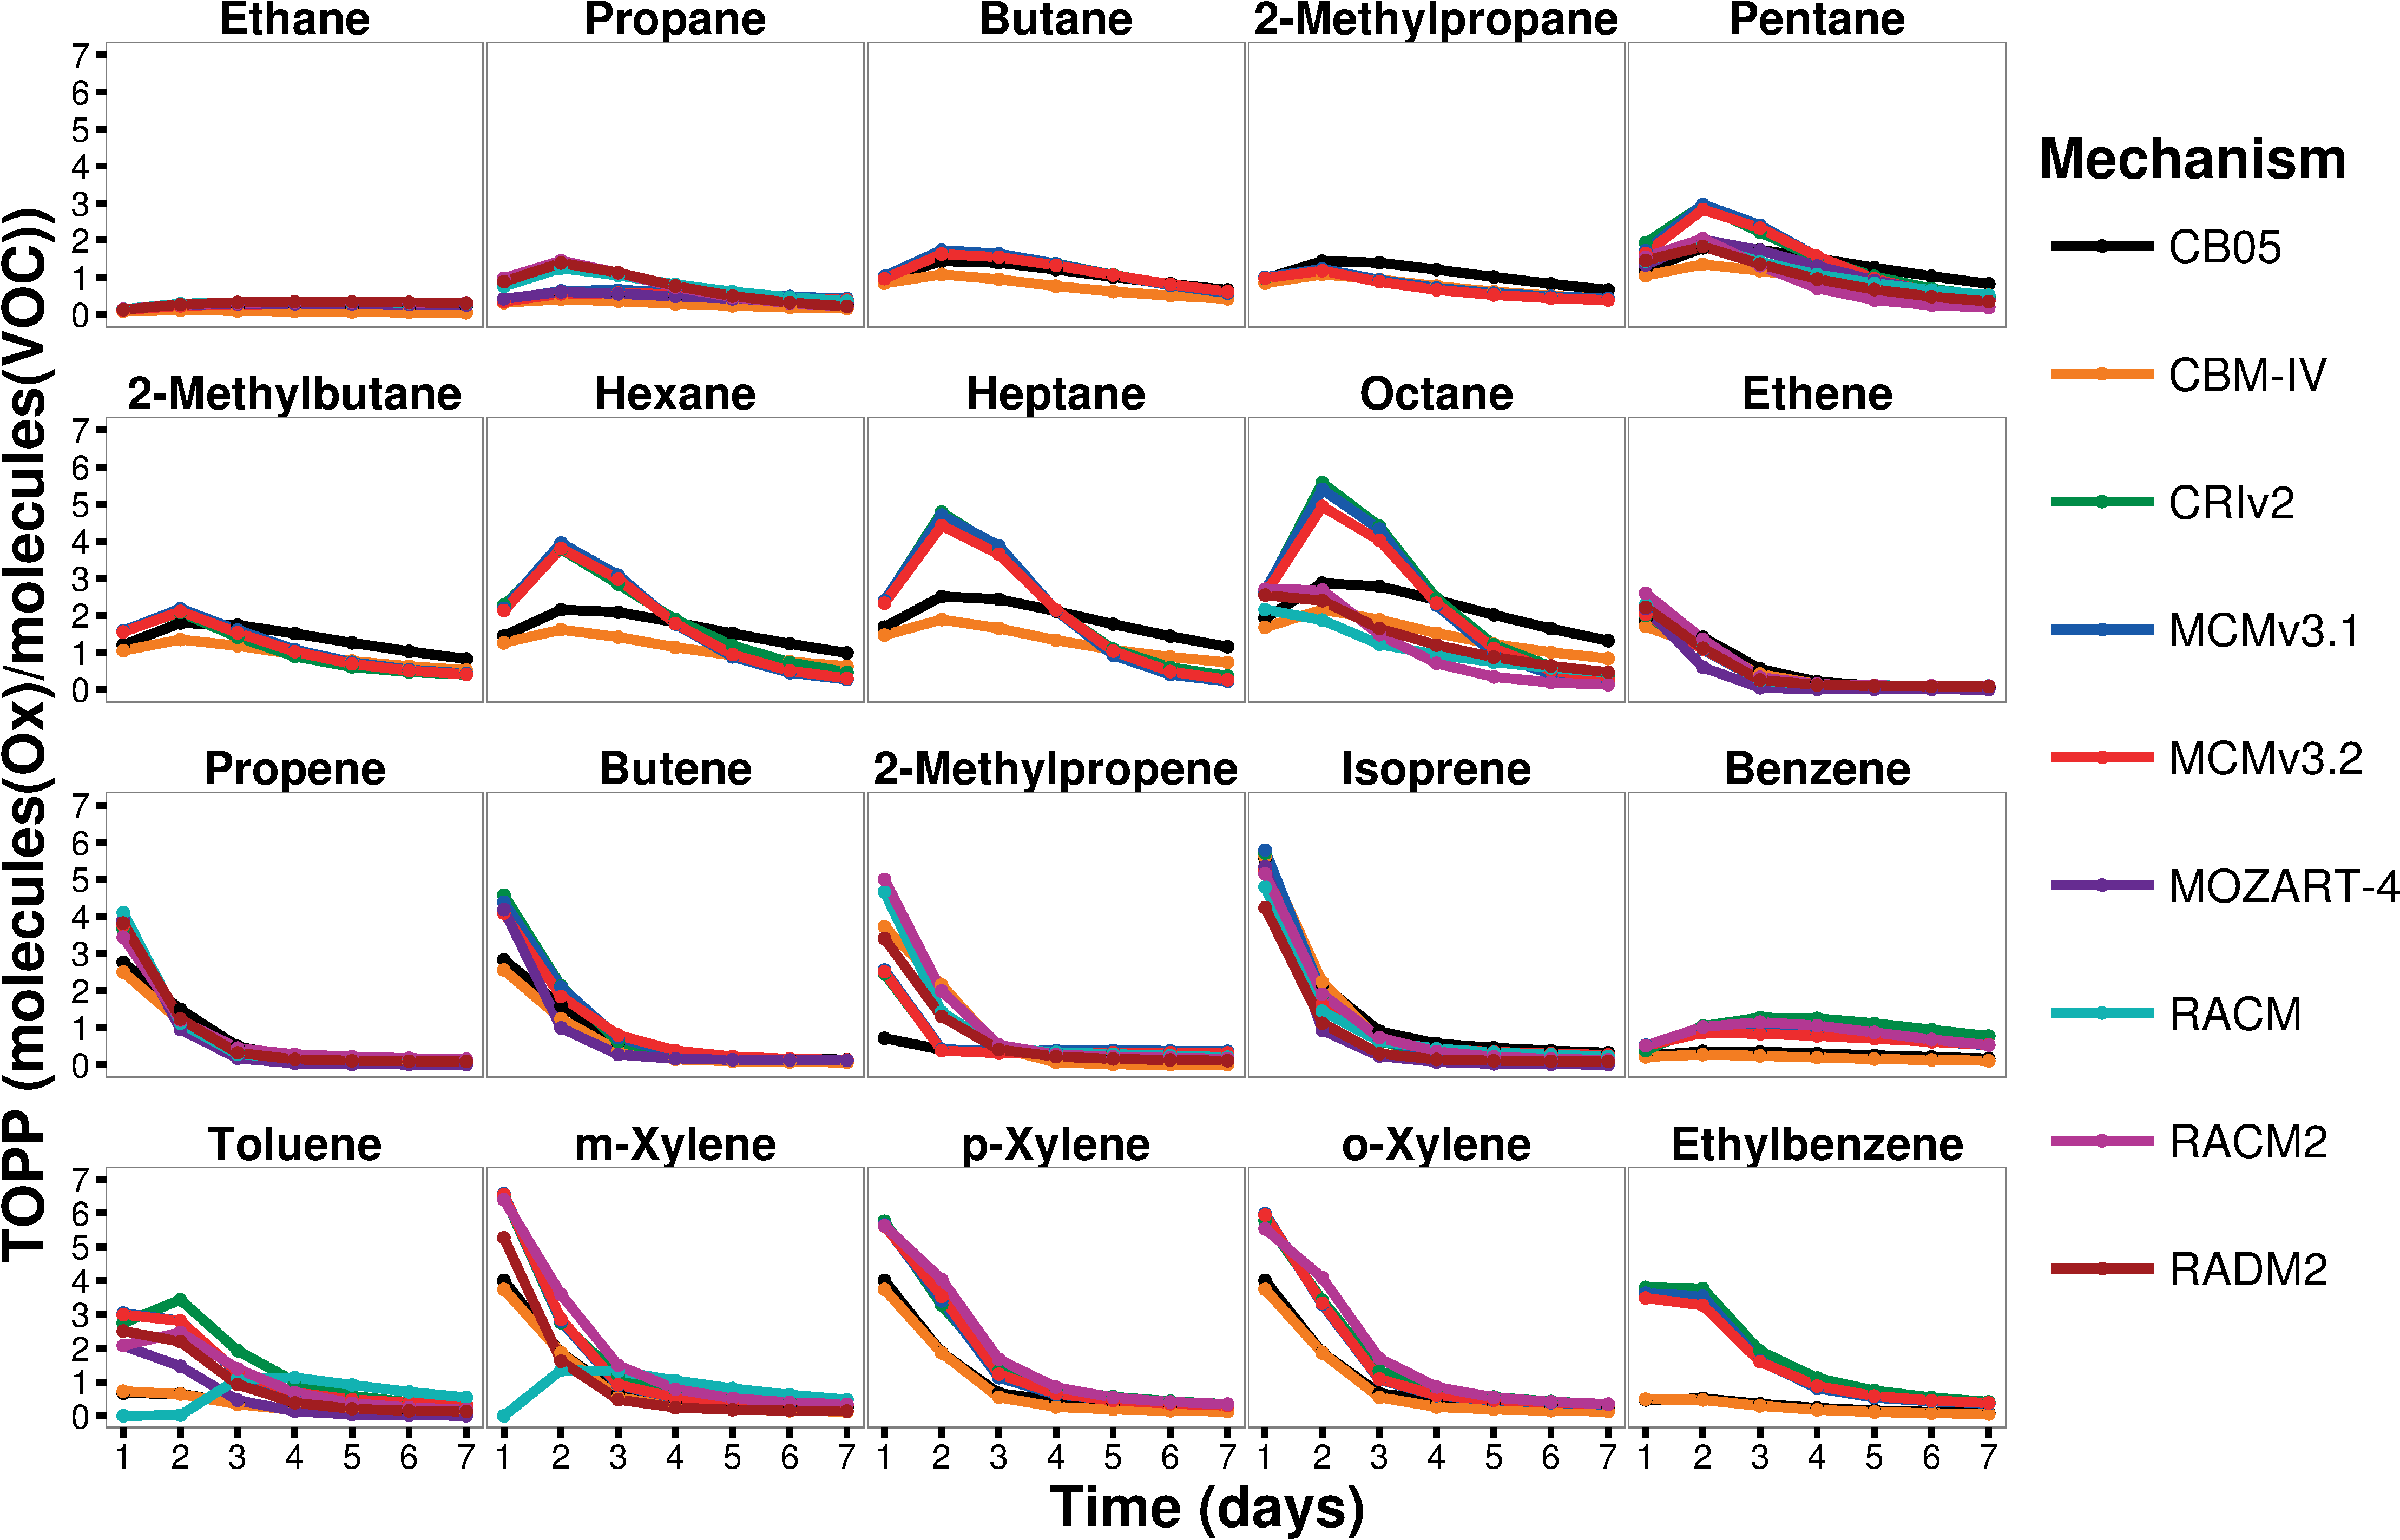
\includegraphics[width=\textwidth]{img/TOPP_daily_values_all_species}
    \end{center}
    \caption{TOPP value time series for all NMVOCs obtained with each mechanism.}
    \label{f:TOPP_dailies}
\end{figure}

The daily TOPP value time series of the considered NMVOCs are presented in \mbox{Figure \ref{f:TOPP_dailies}}. 
NMVOCs, such as ethene, whose degradation is described using dedicated mechanism species show similar time-dependent \ce{O_x} production.
Higher variability emerges between the time series of those NMVOCs represented by lumped mechanism species, such as pentane.

A second day \ce{O_x} production maximum of all alkanes is present by all mechanisms except the RADM2, RACM and RACM2 representations of octane. 
Also, the MCM mechanisms have pronounced maxima that increases with carbon number.

\ce{O_x} production is attributed to the carbon number of the NMVOC degradation products in Section \ref{ss:c_number} demonstrating that the reduced mechanisms break down the emitted NMVOC into species with a lower number of carbon atoms quicker than more detailed mechanisms. 
%possibly re-word this
In the case of octane, this break down proceeds so quickly that its TOPP value maximum is on the first day. 
The supplement to this paper contains details of the octane analysis.

Aromatic VOC \ce{O_x} production shows the highest variability between mechanisms. 
In particular, zero \ce{O_x} production results for both toluene and m-xylene when using RACM, which is explained in Section \ref{sss:RACM_aromatic}. 
The rapid toluene break down in CBM-IV and CB05 results in low \ce{O_x} production throughout the model run.
This impacts the ethylbenzene TOPP value time series since it is represented as \mbox{TOL + PAR}.

\subsubsection{RACM Aromatic Chemistry} \label{sss:RACM_aromatic}

\begin{figure}
    \begin{center}
        \includegraphics[width=\textwidth]{img/TOL_MCM_RACM_Ox_intermediates}
    \end{center}
    \caption{The \ce{O_x} production and consumption budgets from toluene degradation in \mbox{(a) MCM v3.2} and (b) RACM.}
    \label{f:TOL_MCM_RACM}
\end{figure}

The \ce{O_x} production and consumption budgets due to toluene degradation in MCM v3.2 and RACM are depicted in Figure \ref{f:TOL_MCM_RACM}. 
The tagging approach allows attribution of these budgets to the responsible organic reactions.

RACM chemistry results in net \ce{O_x} consumption on the first two days in contrast to the net \ce{O_x} production throughout the MCM v3.2 model run.
This is due to several \ce{O_x}-consuming reactions in RACM which are not present in the MCM, in particular the cresol OH-adduct mechanism species ADDC reaction with \ce{O3}. 
A fast rate constant \mbox{($5 \times 10^{-11}$ cm$^3$ s$^{-1}$)} was assigned to the this reaction making it the main reaction pathway of ADDC. 
This reaction was included in RACM due to improved cresol product yields when comparing RACM predictions with experimental data \citep{Stockwell:1997}.

Other mechanisms that include cresol OH-adduct species do not include reaction with \ce{O3}. 
The inclusion of aromatic OH-adduct species ozonolysis in RACM results in non-representative \ce{O_x} production. 
This has been updated in RACM2 where aromatic OH-adduct species ozonolysis is no longer included.
